\chapter{Implementazione}
Per lo studio di quanto descritto fino ad ora si è costruito un programma che possa caricare un file wav in buffer di dimensione arbitraria in memoria per poterne elaborare il contenuto; dopodiché è possibile specificare una catena di operazioni da effettuare sul segnale e un metodo di salvataggio del risultato (.wav o .csv). La catena di operazioni e il salvataggio vengono specificati in un file di testo. Per la lettura e scrittura su file .wav si utilizza la libreria ``libsndfile'' scritta da Erik de Castro Lopo\cite{libsndfile}.

\section{Strutture dati utilizzate}

Per la rappresentazione dei dati si utilizza una struttura nominata \lstinline{SignalBuffer_t} definita nel seguente modo:

\begin{lstlisting}
struct SignalBuffer_t
{
	cuComplex* samples;
	size_t channels;
	size_t* channel_size;
	size_t max_size;
};
\end{lstlisting}

Essa continene un array di campioni, il numero di canali, la lunghezza dei buffer di ogni canale e la lunghezza massima disponibile dell'array. A prima vista può sembrare strana ma è necessaria questa configurazione per facilitare le operazioni di input/output dei file wav e soprattutto le operazioni di trasporto della memoria dalla e alla GPU.

\lstinline{cuComplex} è un tipo importato dalla libreria di cuda il quale rappresenta un numero complesso. Esso può essere utilizzato, con le apposite operazioni, sia dalla CPU sia dalla GPU.

Vengono definite anche operazioni su questa struttura, di cui viene riportata l'implementazione delle due principali. Tutte le funzioni sono dichiarate con i modificatori \lstinline{__host__ __device__ inline} per segnalare che sono funzioni che possono essere usate sia dalla cpu, sia dalla gpu; inoltre sono inline per snellire la loro chiamata in quanto sono usate spesso.

\begin{lstlisting}
    size_t get_channels(SignalBuffer_t buffer)
    size_t get_channel_buffer_size(SignalBuffer_t buffer, size_t channel);
    size_t get_max_buffer_size(SignalBuffer_t buffer);
    size_t get_max_channel_buffer_size(SignalBuffer_t buffer);
    size_t get_max_possible_channel_buffer_size(SignalBuffer_t buffer, size_t channel);
    int set_channel_buffer_size(SignalBuffer_t buffer, size_t channel, size_t size);
    size_t get_signal_buffer_channel_sample_index(SignalBuffer_t buffer, size_t channel, size_t index)
    {
	return index * buffer.channels + channel;
    }

    cuComplex get_signal_buffer_sample(SignalBuffer_t buffer, size_t channel, size_t index)
    {
        size_t buffer_size = get_channel_buffer_size(buffer, channel);
        if (index >= buffer_size)
            return make_cuComplex(0, 0);
        return buffer.samples[get_signal_buffer_channel_sample_index(buffer, channel, index)];
    }
    
    int set_signal_buffer_sample(SignalBuffer_t buffer, size_t channel, size_t index, cuComplex value)
    {
        size_t current_buffer_size = get_channel_buffer_size(buffer, channel);
        if (index >= current_buffer_size)
        {
            size_t new_current_buffer_size = index + 1;
            if (!set_channel_buffer_size(buffer, channel, new_current_buffer_size)) {
                // buffer overflow
                return 0;
            }
        }
        buffer.samples[get_signal_buffer_channel_sample_index(buffer, channel, index)] = value;
    
        return 1;
    }

\end{lstlisting}

\section{DFT}
\subsection{CPU}
L'operazione di trasformata di Fourier discreta è implementata sulla CPU nel seguente modo:

\begin{lstlisting}
void dft_wsio(SignalBuffer_t* bufferIn, SignalBuffer_t* bufferOut, size_t channel, size_t size)
{
	cuComplex* tmp = new cuComplex[size];
	cuComplex sample, s;
	for (size_t k = 0; k < size; k++)
	{
		tmp[k] = make_cuFloatComplex(0,0);
		for (size_t i = 0; i < size; i++)
		{
			s = cuComplex_exp(-2 * M_PI * k * i / size);
			sample = get_signal_buffer_sample(*bufferIn, channel, i);
			tmp[k] = cuCaddf(tmp[k], cuCmulf(sample, s));
		}
	}
	for (size_t k = 0; k < size; k++)
	{
		set_signal_buffer_sample(*bufferOut, channel, k, tmp[k]);
	}
	delete[] tmp;
}
\end{lstlisting}

\lstinline{cuComplex_exp(float x)} è una funzione che restituisce il numero complesso $e^{jx}$. L'algoritmo prende in input un buffer di cui effettuare la trasformata, un buffer in cui inserire il risultato della trasformazione, il canale dei buffer su cui operare e la dimensione in punti della trasformata. Come esposto in precedenza la funzione \lstinline{get_signal_buffer_sample} restituisce il numero complesso $0$ nel caso il valore dell'indice sia fuori range. Questo permette di implementare facilmente la dft di un buffer con un pad di zeri alla sua destra.

\begin{figure}[h]
    \centering
    \subfloat[Impulso]{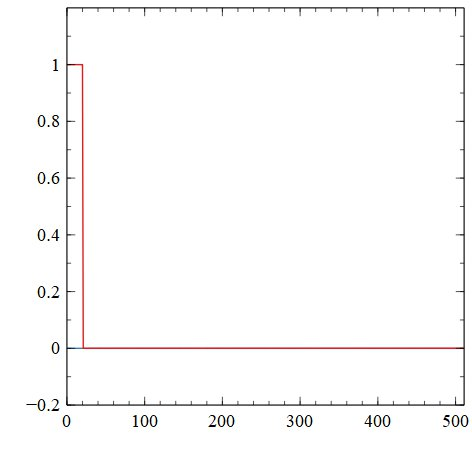
\includegraphics[width=0.5\textwidth]{pulse512}}
    \subfloat[Dft]{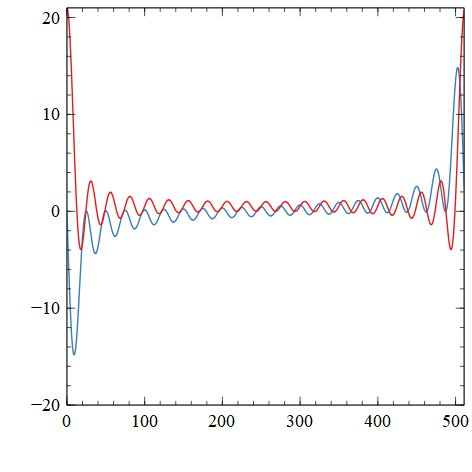
\includegraphics[width=0.5\textwidth]{pulse512dft}}
    \caption{DFT di un impulso. In rosso è segnata la parte reale e in blu la parte immaginaria}
    \label{fig:pulse512}
\end{figure}

Inserendo nel programma l'impulso di 512 campioni mostrato in figura \ref{fig:pulse512}a si ottiene la trasformata in figura \ref{fig:pulse512}b. Come è facile notare, il segnale di partenza ha solo componente reale, quindi la sua trasformata è simmetrica rispetto a $N/2$ in modo pari per la parte reale e in modo dispari per la parte immaginaria.

\subsection{GPU}
L'operazione di trasformata di Fourier discreta è implementata sulla GPU utilizzando i seguenti kernel:

\begin{lstlisting}
__global__ void cudadft_kernel_dft(SignalBuffer_t device_buffer, SignalBuffer_t tmp, size_t channel)
{
    int k = blockIdx.x * blockDim.x + threadIdx.x;
    size_t size = get_channel_buffer_size(device_buffer, channel);
    cuComplex temp = make_cuComplex(0, 0);
    cuComplex sample, s;
    
    for (int i = 0; i < size; i++)
    {
        sample = get_signal_buffer_sample(device_buffer, channel, i);

        s = cuComplex_exp(-2.0f * PI * k * i / size);

        temp = cuCaddf(temp, cuCmulf(sample, s));
    }
    
    set_signal_buffer_sample(tmp, channel, k, temp);
}

__global__ void cudadft_kernel_copy(SignalBuffer_t device_buffer, SignalBuffer_t tmp, size_t channel)
{
    int k = blockIdx.x * blockDim.x + threadIdx.x;
    cuComplex sample = get_signal_buffer_sample(tmp, channel, k);
    set_signal_buffer_sample(device_buffer, channel, k, sample);
}
\end{lstlisting}

Il primo kernel si occupa di calcolare la DFT del segnale, mentre il secondo è un kernel che viene eseguito dopo che tutti i thread del primo sono completati e si occupa di ricopiare il risultato della dft da tmp al buffer originario. È necessaria questa divisione di compiti per evitare che vengano scritti dei valori nel buffer originario prima che tutti i thread abbiano finito di accedervi. Inserendo l'impulso di figura \ref{fig:pulse512}a nel programma con dft in CUDA si ottiene lo stesso risultato di \ref{fig:pulse512}b.

\section{Fast Fourier Transform}
L'operazione di DFT è onerosa in termini di calcolo in quanto ha complessita $O(N^2)$, per cui si utilizza spesso la Fast Fourier Transform al suo posto (FFT). Uno degli algoritmi più popolari per il calcolo della FFT è quello ideato da Cooley e Tukey nel 1965. Esso fa uso della decomposizione interlacciata e delle somme a ``farfalla''.

[da espandere con più info]

\subsection{CPU}
La FFT è implementata sulla CPU nel seguente modo:

\begin{lstlisting}
    void fft_wsio(SignalBuffer_t* bufferIn, SignalBuffer_t* bufferOut, size_t channel, size_t size_in)
    {
        cuComplex w, wm;
        size_t levels;
        size_t index_a, index_b;
        size_t size = (size_t)pow(2, ceil(log2(size_in)));;
        levels = (size_t)log2(size);
        bit_reversal_sort_wsio(bufferIn, bufferOut, channel, size);
        for (size_t level = 0; level < levels; level++)
        {
            size_t butterflies_per_dft = (size_t)pow(2, level);
            size_t dfts = size / (butterflies_per_dft * 2);
            wm = cuComplex_exp(-(M_PI / butterflies_per_dft));
            w = make_cuComplex(1,0);
            for (size_t butterfly = 0; butterfly < butterflies_per_dft; butterfly++)
            {
                for (size_t dft = 0; dft < dfts; dft++)
                {
                    index_a = butterfly + dft * (butterflies_per_dft * 2);
                    index_b = index_a + butterflies_per_dft;
                    cuComplex a = get_signal_buffer_sample(*bufferOut, channel, index_a);
                    cuComplex b = get_signal_buffer_sample(*bufferOut, channel, index_b);
                    butterfly_calculation(&a, &b, w);
                    set_signal_buffer_sample(*bufferOut, channel, index_a, a);
                    set_signal_buffer_sample(*bufferOut, channel, index_b, b);
                }
                w = cuCmulf(w, wm);
            }
        }
    }
\end{lstlisting}

Le funzioni \lstinline{bit_reversal_sort_wsio} e \lstinline{butterfly_calculation} sono consultabili in appendice.

[Più info su come funziona].

\subsection{GPU}

[da fare]

\section{Convoluzione}
[info]
\subsection{CPU}
La convoluzione è implementata sulla CPU nel seguente modo:

\begin{lstlisting}
    size_t buffer_size = get_channel_buffer_size(*buffer, channel);
    size_t signal_size = get_channel_buffer_size(this->signal, SIGNAL_CHANNEL);
    size_t remaining_samples = this->samples_remaining[channel];

    size_t temp_index = this->temp_indexes[channel];
    if ((buffer_size == 0 || signal_size == 0) && remaining_samples > 0)
    {
        size_t count = 0;
        cuComplex sample = get_signal_buffer_sample(this->temp, channel, temp_index);
        while (remaining_samples > 0 &&
            set_signal_buffer_sample(*buffer, channel, count, sample)) {

            count++;
            temp_index = bounded_index(this->temp, channel, temp_index + 1);
            sample = get_signal_buffer_sample(this->temp, channel, temp_index);
            remaining_samples--;
        }
        temp_indexes[channel] = temp_index;
        samples_remaining[channel] = remaining_samples;
        continue;
    }
    size_t total = buffer_size + signal_size - 1;
    for (size_t i = 0; i < buffer_size; i++)
    {
        cuComplex in_sample = get_signal_buffer_sample(*buffer, channel, i);
        for (size_t j = 0; j < signal_size; j++)
        {
            cuComplex signal_sample = get_signal_buffer_sample(this->signal, SIGNAL_CHANNEL, j);
            size_t index = bounded_index(this->temp, channel, temp_index + i + j);
            cuComplex out_sample = get_signal_buffer_sample(this->temp, channel, index);
            cuComplex result = cuCaddf(out_sample, cuCmulf(in_sample, signal_sample));
            set_signal_buffer_sample(this->temp, channel, index, result);
        }
    }
    for (size_t i = 0; i < buffer_size; i++)
    {
        size_t index = bounded_index(this->temp, channel, temp_index + i);
        cuComplex out_sample = get_signal_buffer_sample(this->temp, channel, index);
        set_signal_buffer_sample(*buffer, channel, i, out_sample);
        set_signal_buffer_sample(this->temp, channel, index, make_cuComplex(0, 0));
    }
    this->temp_indexes[channel] = bounded_index(this->temp, channel, temp_index + buffer_size);
    this->samples_remaining[channel] = signal_size - 1;
\end{lstlisting}


\subsection{GPU}
Sulla GPU si utilizzano i seguenti kernel.
\begin{lstlisting}
__global__ void cudaconvolver_kernel_output(SignalBuffer_t device_buffer, SignalBuffer_t signal, SignalBuffer_t tmp, size_t channel, size_t temp_index)
{
	int k = blockIdx.x * blockDim.x + threadIdx.x;
	size_t out_size = get_channel_buffer_size(tmp, channel);
	if (k >= out_size)
		return;
	size_t signal_size = get_channel_buffer_size(signal, SIGNAL_CHANNEL);
	cuComplex temp = make_cuComplex(0, 0);
	cuComplex signal_sample, input_sample;
	size_t index = cuda_bounded_index(tmp, channel, temp_index + k);
	cuComplex temp_sample = get_signal_buffer_sample(tmp, channel, index);
	for (int i = 0; i < signal_size; i++)
	{
		signal_sample = get_signal_buffer_sample(signal, SIGNAL_CHANNEL, i);
		if (i > k)
			input_sample = make_cuComplex(0,0);
		else
			input_sample = get_signal_buffer_sample(device_buffer, channel, k-i);
		temp_sample = cuCaddf(temp_sample, cuCmulf(signal_sample, input_sample));
	}
	set_signal_buffer_sample(tmp, channel, index, temp_sample);
}
__global__ void cudaconvolver_kernel_copy(SignalBuffer_t device_buffer, SignalBuffer_t tmp, size_t channel, size_t temp_index)
{
	int k = blockIdx.x * blockDim.x + threadIdx.x;

	size_t tmp_size = get_channel_buffer_size(tmp, channel);
	size_t out_size = get_channel_buffer_size(device_buffer, channel);
	if (k >= tmp_size)
		return;

	size_t index = cuda_bounded_index(tmp, channel, temp_index + k);
	cuComplex sample = get_signal_buffer_sample(tmp, channel, index);
	set_signal_buffer_sample(device_buffer, channel, k, sample);
	if (k < out_size)
		set_signal_buffer_sample(tmp, channel, index, make_cuComplex(0,0));
}
\end{lstlisting}

In figura \ref{fig:pulse32conv} si può apprezzare una convoluzione di un impulso di 32 campioni con se stesso ottenuto dagli algoritmi presentati.

\begin{figure}[h]
    \centering
    \subfloat[Impulso]{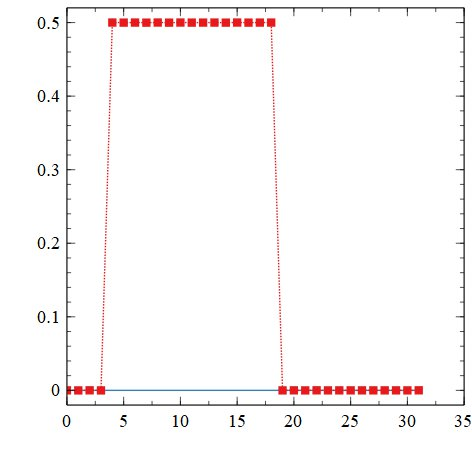
\includegraphics[width=0.5\textwidth]{pulse32}}
    \subfloat[Convoluzione]{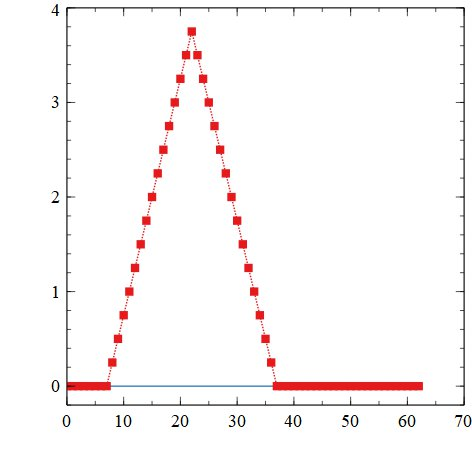
\includegraphics[width=0.5\textwidth]{pulse32conv}}
    \caption{Convoluzione di un impulso rettangolare con sé stesso. In rosso è segnata la parte reale e in blu la parte immaginaria}
    \label{fig:pulse32conv}
\end{figure}